\newpage
\section{Графики и картинки с результатами}

\begin{figure}[h] % here, top, bottom, page
    \centering
    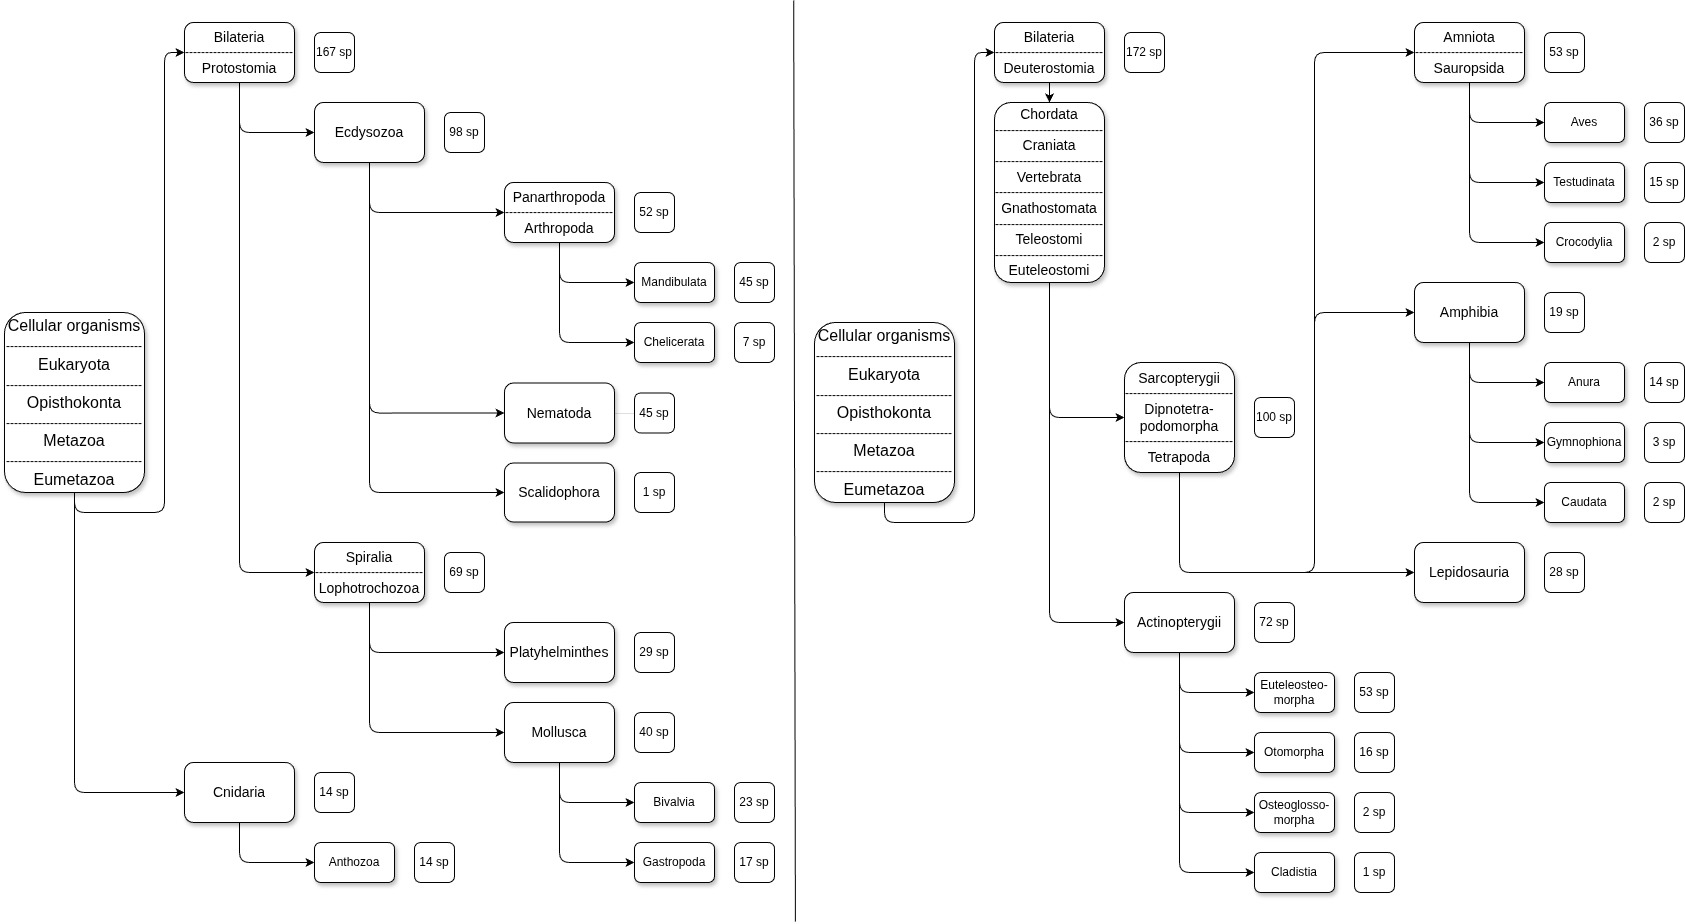
\includegraphics[width=1.0\textwidth]{images/Tree_summary}
    \caption{Количество видов, взятых в анализ для Protostomia+Cnidaria и Deuterostomia.}
    \label{fig:tree_1}
\end{figure}

\newpage
\begin{figure}[h] % here, top, bottom, page
    \centering
    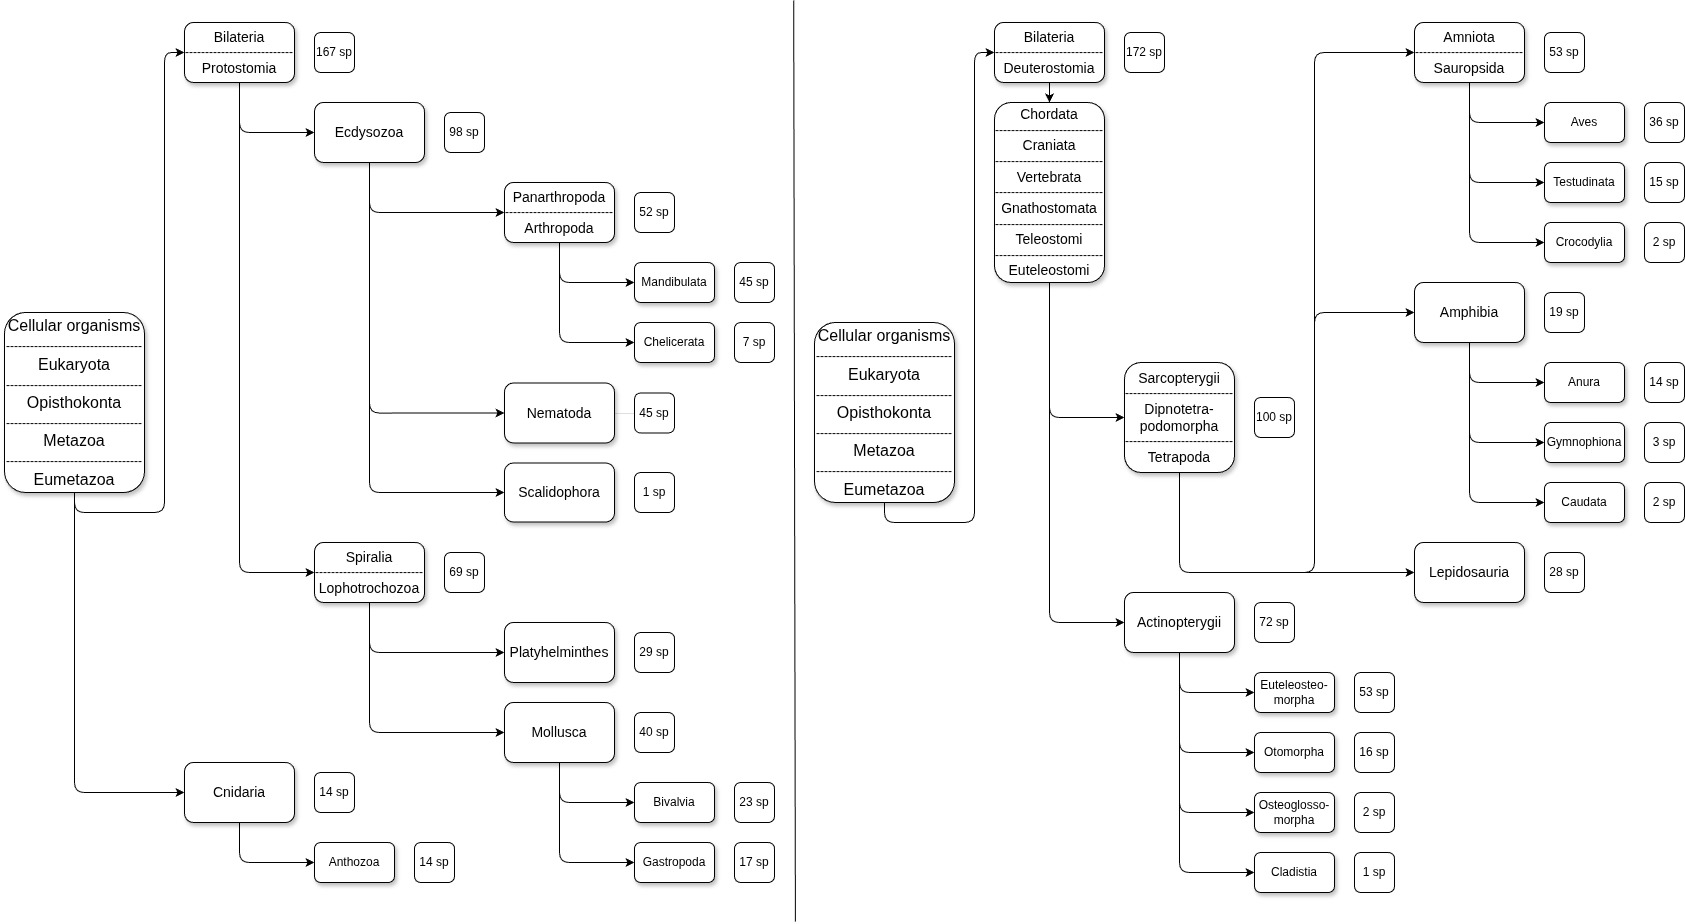
\includegraphics[width=1.0\textwidth]{images/Tree_summary_v2}
    \caption{Количество видов, взятых в анализ для Protostomia+Cnidaria и Deuterostomia.}
    \label{fig:tree_2}
\end{figure}

\newpage
\begin{figure}[h] % here, top, bottom, page
    \centering
    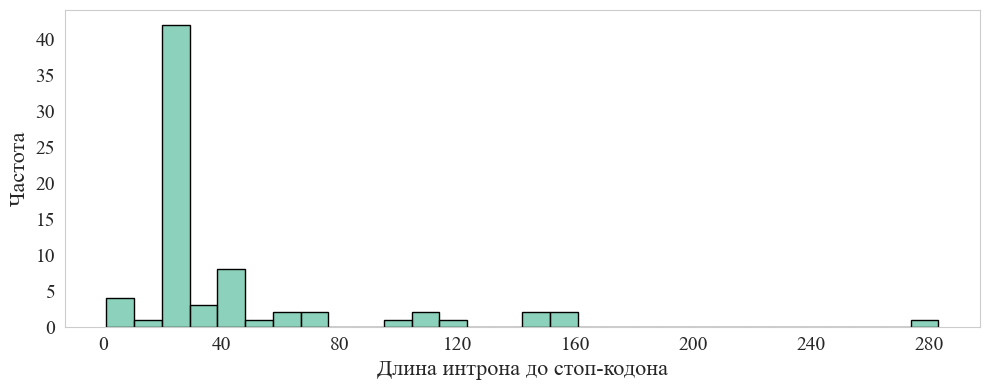
\includegraphics[width=1.0\textwidth]{images/Actinopterygii_intron_stop}
    \caption{Распределение длин части кассетного интрона до стоп-кодона у таксономической группы Actinopterygii}
    \label{fig:Actinopterygii_intron_stop}
\end{figure}

\newpage
\begin{figure}[h] % here, top, bottom, page
    \centering
    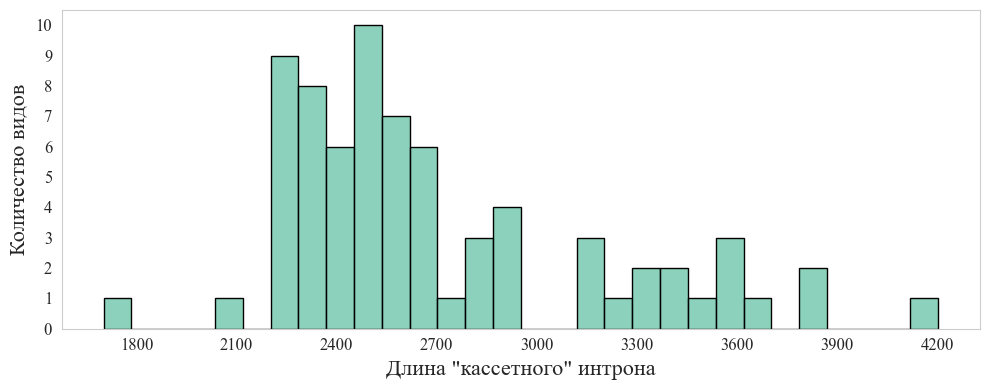
\includegraphics[width=1.0\textwidth]{images/Actinopterygii_intron}
    \caption{Распределение длин кассетного интрона у таксономической группы Actinopterygii}
    \label{fig:Actinopterygii_intron}
\end{figure}


\newpage
\begin{figure}[h] % here, top, bottom, page
    \centering
    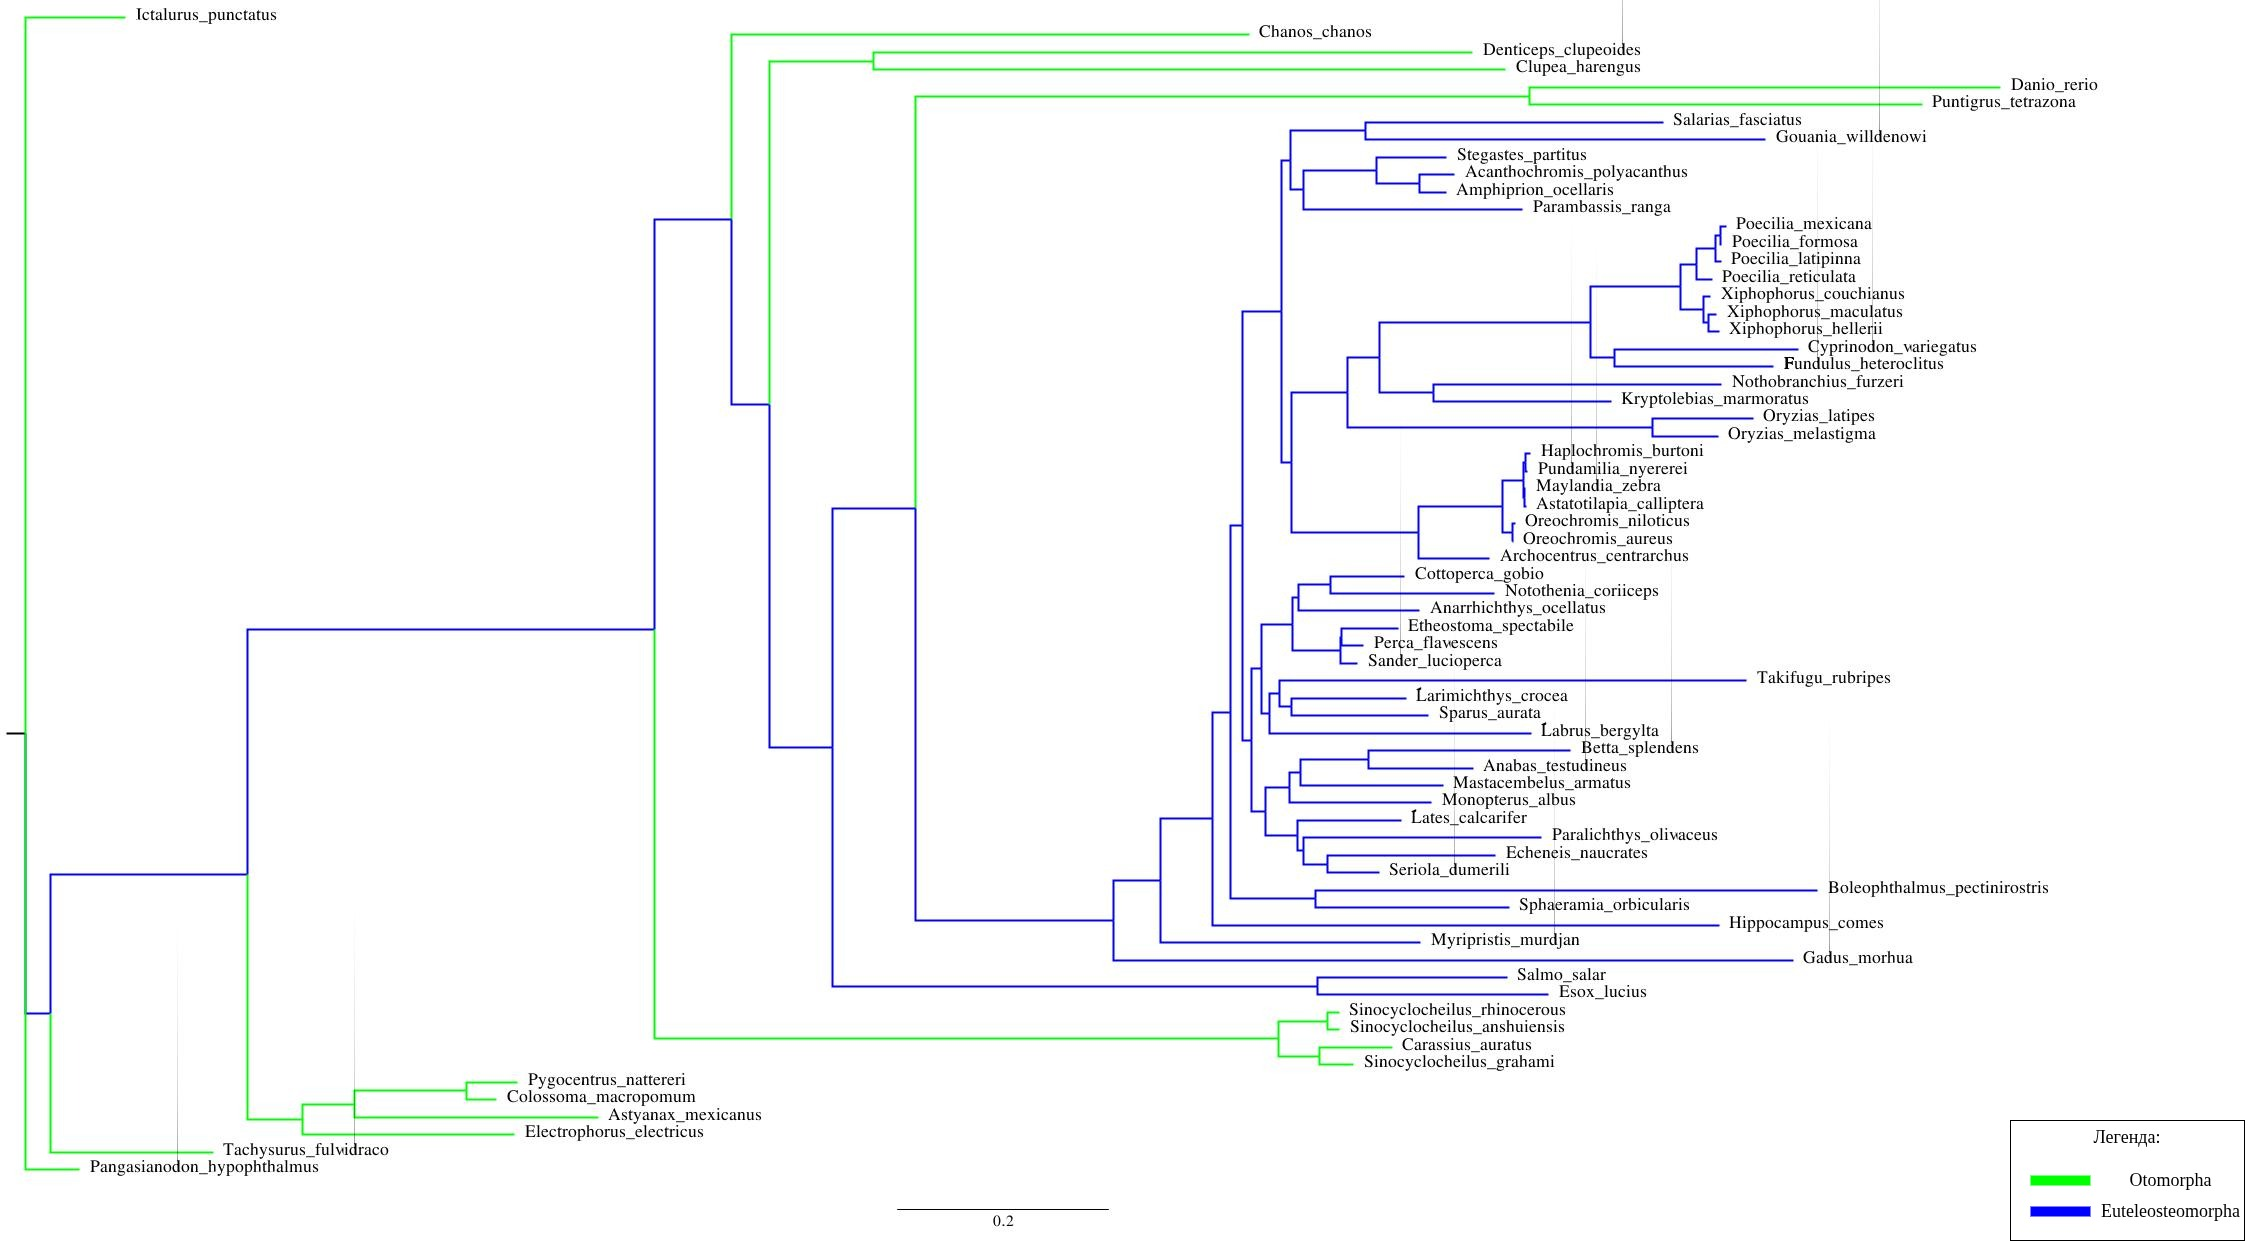
\includegraphics[width=1.0\textwidth]{images/Actinopterygii_tree}
    \caption{Филогенетическое дерево для таксономической группы Actinopterygii}
    \label{fig:Actinopterygii_tree}
\end{figure}


\newpage
\begin{figure}[h] % here, top, bottom, page
    \centering
    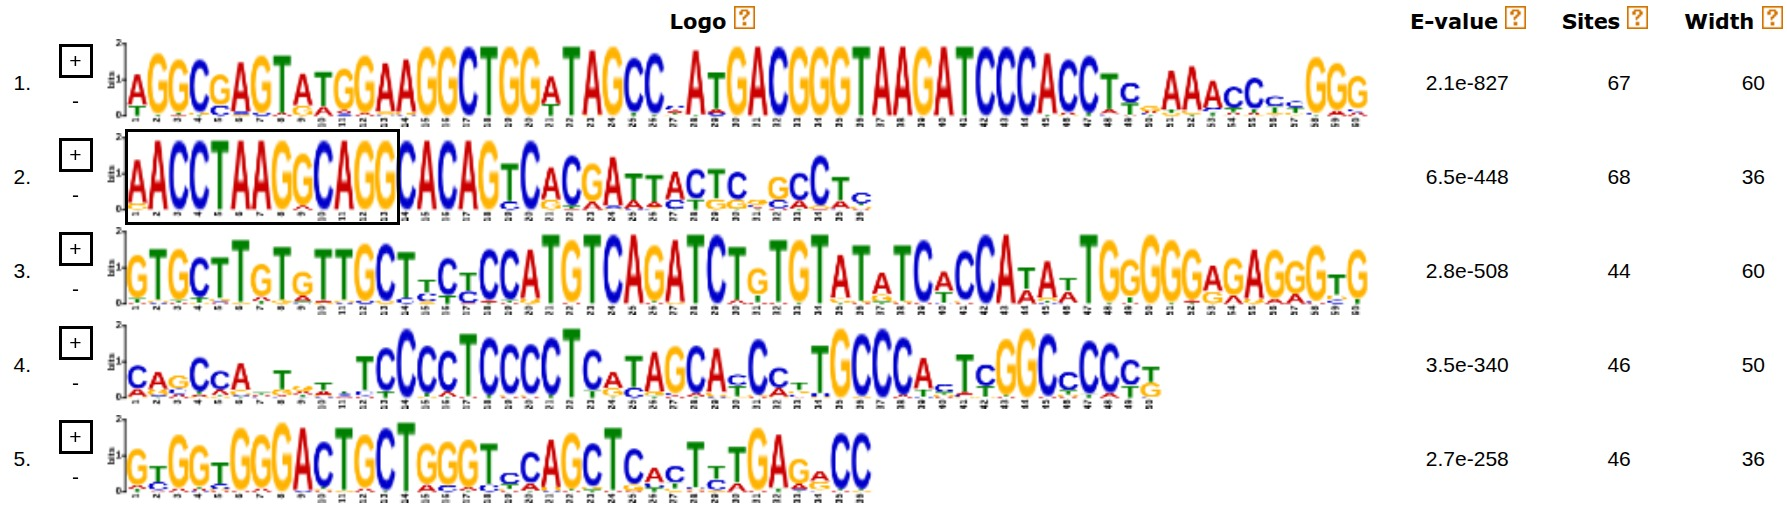
\includegraphics[width=1.0\textwidth]{images/Actinopterygii_meme_motif}
    \caption{Результат поиска мотивов внутри кассетного интрона с помощью meme для таксономической группы Actinopterygii.\\
    Черным прямоугольником выделен участок, похожий на консенсусную последовательность CTE из статьи 2001 года.}
    \label{fig:Actinopterygii_meme}
\end{figure}


\begin{figure}[h] % here, top, bottom, page
    \centering
    
\includegraphics[width=0.8\textwidth]{images/CTE_consensus}
    \caption{Консенсусный CTE из статьи 2001 года}
    \label{fig:CTE_consensus}
\end{figure}


\newpage
\begin{figure}[h] % here, top, bottom, page
    \centering
    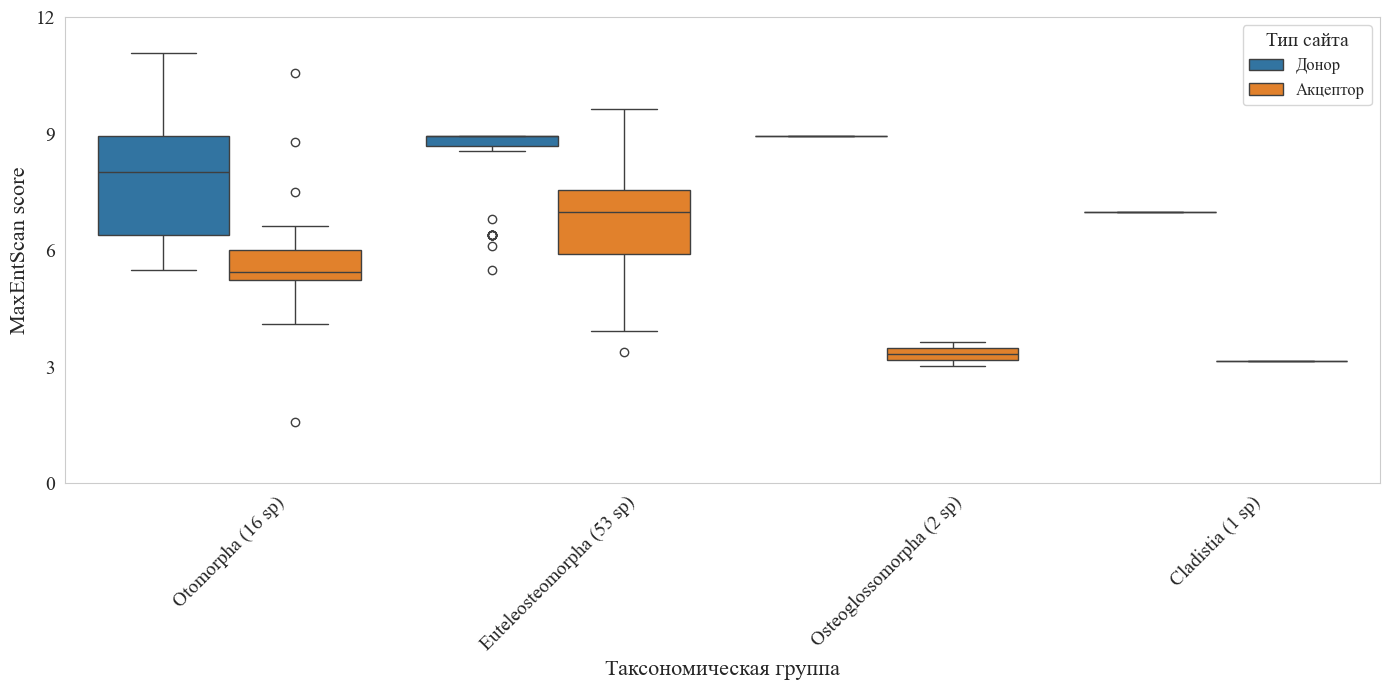
\includegraphics[width=1.0\textwidth]{images/Actinopterygii_maxentscan}
    \caption{Результаты проведения MaxEntScan для 72 видов из Actinopterygii.}
    \label{fig:Actinopterygii_maxentscan}
\end{figure}

\newpage
\begin{figure}[h] % here, top, bottom, page
    \centering
    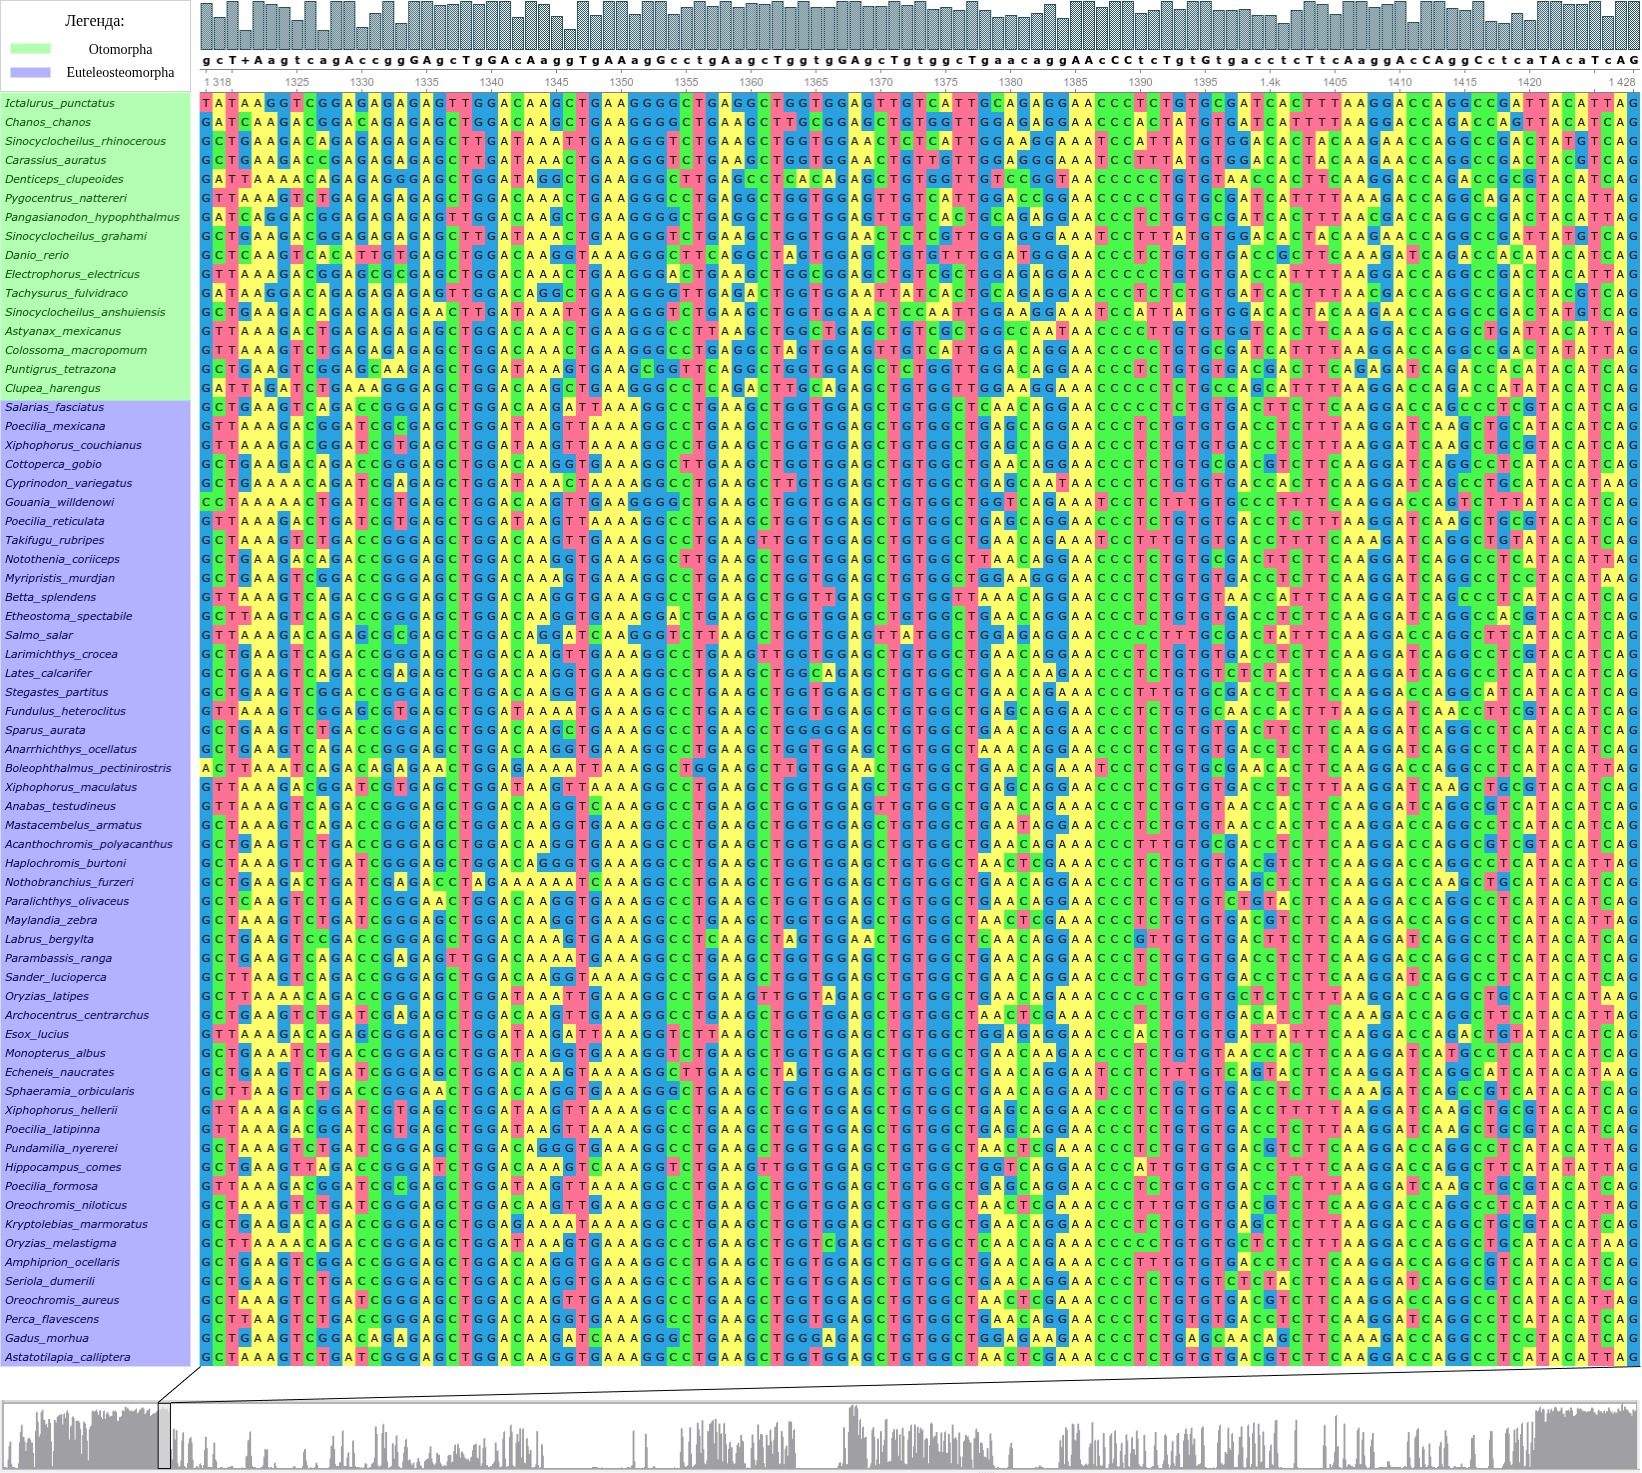
\includegraphics[width=1.0\textwidth]{images/Actinopterygii_alignment_ruler}
    \caption{Результаты множественного выравнивания для 72 видов из Actinopterygii.}
    \label{fig:Actinopterygii_alignment_ruler}
\end{figure}


\newpage
\begin{figure}[h] % here, top, bottom, page
    \centering
    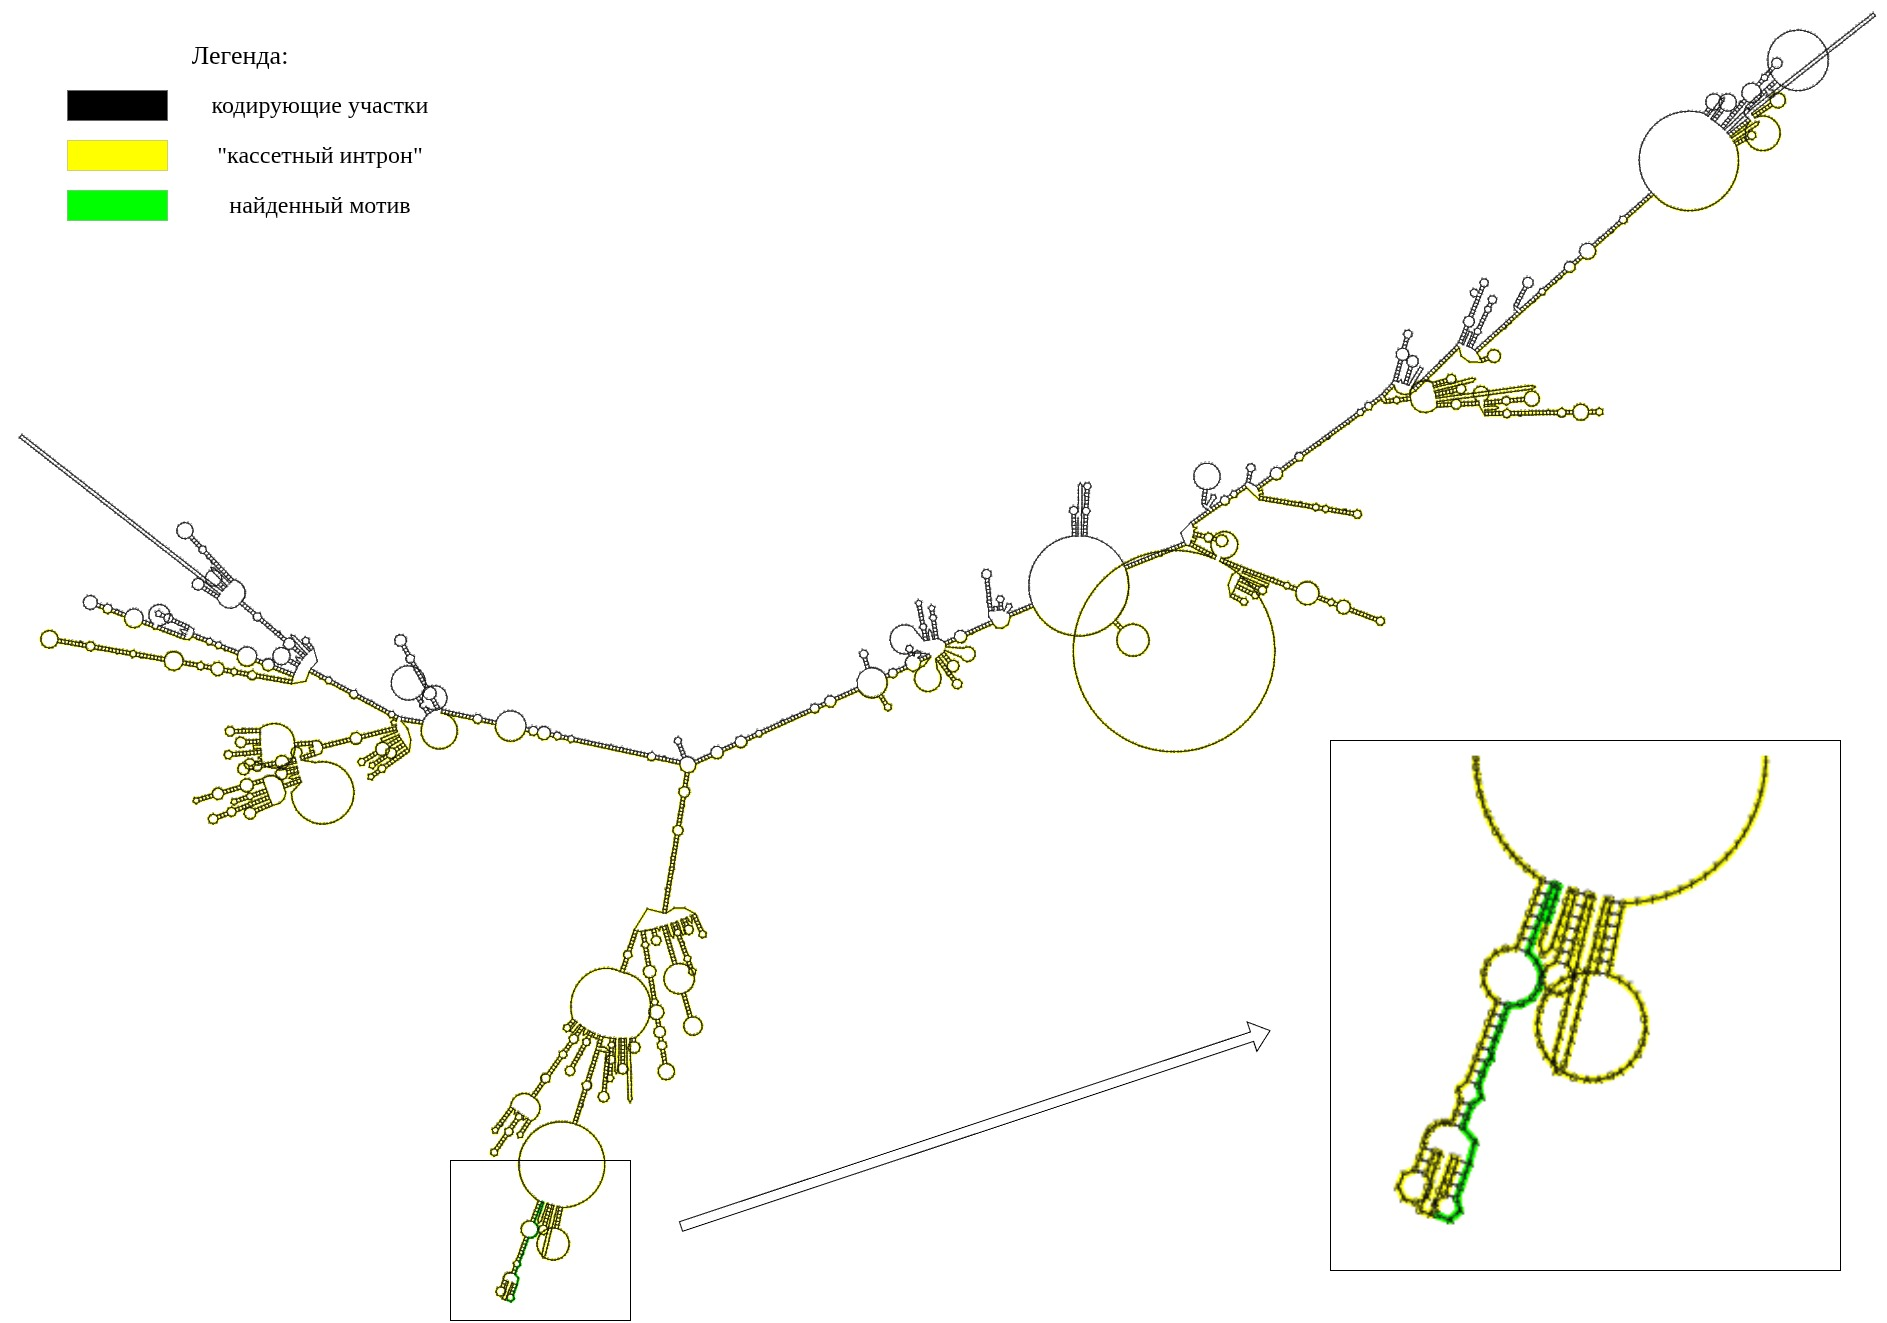
\includegraphics[width=1.0\textwidth]{images/Chanos_chanos_2nd_structure}
    \caption{Вторичная структура РНК-транскрипта для \textit{Chanos chanos} из Otomorpha, содержащая кассетный интрон.}
    \label{fig:Chanos_chanos_2nd_structure}
\end{figure}
